\documentclass[12pt, a4paper,oneside]{article}

\usepackage{graphicx}
\graphicspath{ {references/} }


\usepackage{float}%figures placed HERE

\usepackage[backend=bibtex]{biblatex}
\bibliography{miniproject}
%\bibliographystyle{plain}


\title{Reconfigurable and Low Energy Systems Miniproject\\\large CORDIC}
\author{Anders Normann Poulsen (apouls16@student.aau.dk)\\Gabriel Vasluianu (gvaslu16@student.aau.dk)}


\begin{document}

\maketitle
\newpage
\section{Introduction}
CORDIC is an algorithm that computes trigonometric functions (and many other)
by using simple operations.
%https://en.wikipedia.org/wiki/CORDIC
A typical application would be a two-dimensional vector rotation, as seen in 
figure \ref{fig:two_vector}. Here $(x_{in}, y_{in})$ are the initial coordinates
of the vector, and $(x_{out}, y_{out})$ are the final coordinates.

\begin{figure}[h]
	\centering
	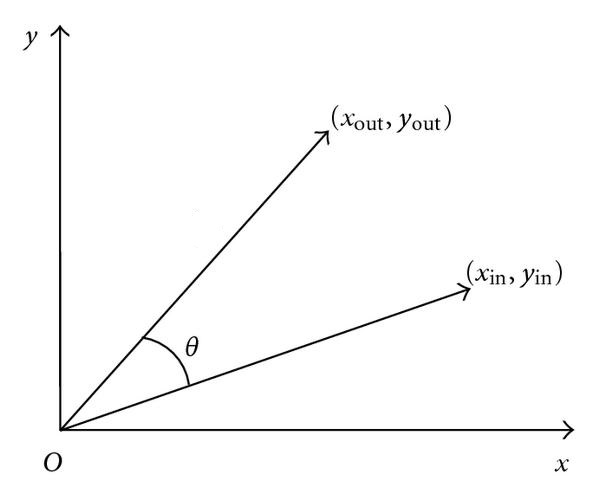
\includegraphics[width = 7cm]{two_vector.jpg}
	\caption{Two dimensional vector rotation}
	\label{fig:two_vector}
\end{figure}

In order to achieve the operation of rotating the vector, the following equations
have to be calculated:
\[ x_{out} = x_{in} cos\theta - y_{in} sin\theta \]
\[ y_{out} = x_{in} sin\theta + y_{in} cos\theta \]

As seen here, the hardware computing these equations would have to do:
four multiplications, two addition/subtraction 
and access a lookup table for the trigonometric functions\cite{cordic1}.
Keep in mind that multiplication is an expensive operation, and a multiplicator
takes a large area. This is the reason why we want to use CORDIC in some 
applications.
\\

The idea CORDIC introduces is that we can compute the new coordinates by 
iterating through an algorithm that constantly tries to get closer to the 
final result, using a table containing angles to be used in the next iteration
(micro-rotation). These angles can be either added or subtracted in order
to take the next step, and approximate the target, as seen in figure \ref{fig:cordic_iterations}.

\begin{figure}[h]
	\centering
	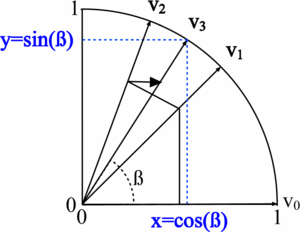
\includegraphics[width = 7cm]{cordic_iterations.png}
	\caption{Ilustration of cordic iterations. V3 is the desired rotation for V0,
	while V1 and V2 are the approximation steps CORDIC takes}
	\label{fig:cordic_iterations}
\end{figure}

The generalized equations of the CORDIC algorithm are:
\[ x_{i+1} = x_i - \sigma_i \cdot 2^{-i} \cdot y_i \]
\[ y_{i+1} = \sigma_i \cdot 2^{-i} \cdot x_i + y_i\]
\[ z_{i+1} = z_i - \sigma_i \cdot arctan(2^{-i}) \]

%https://en.wikibooks.org/wiki/Trigonometry/For_Enthusiasts/The_CORDIC_Algorithm

Here, $x_{i+1}$ and $y_{i+1}$ show us the values respective to each iteration.
In order to know what to do in the next iteration (add/subtract from the previous
angle), we need to compute $\sigma_i$. This is done by looking at the value of 
$z_i$:

$$
\sigma_i = \left\{ \begin{array}{rl}
 +1 &\mbox{ if $z_i>=0$} \\
 -1 &\mbox{ if $z_i<0$}
       \end{array} \right.
$$

$z_i$ keeps track of how much we rotated at every iteration and subtracting that 
from the wanted angle.
The values of $x_i$ and $y_i$ need to be scaled by a factor of $K_i$:

$$K_i = \frac{1}{\sqrt{1 + 2^{-2i}}}$$

However, there are several methods to do this by calculating it in advance or by 
making it a constant. For small architectures, this aspect can be disregarded.
\\
These being said, by looking at the equations we can see that we will need 
to apply the following operations: addition, bitshift and comparison.

\section{From algorithm to architecture}

\subsection{Data flow graph (DFG)}
The data flow graph in figure \ref{fig:cordic_dfg} presents the data dependencies
in the CORDIC algorithm. There are two bit shifting operations, and three
addition/subtraction operations. 

%More information about how these operations
%are executed can be found in \ref{ssec:cdfg}. 

The group had difficulties 
in completely understanding how the interdependency between $x_{i+1}$
and $y_{i+1}$ will affect the architecture of the system.

\begin{figure}[H]
	\centering
    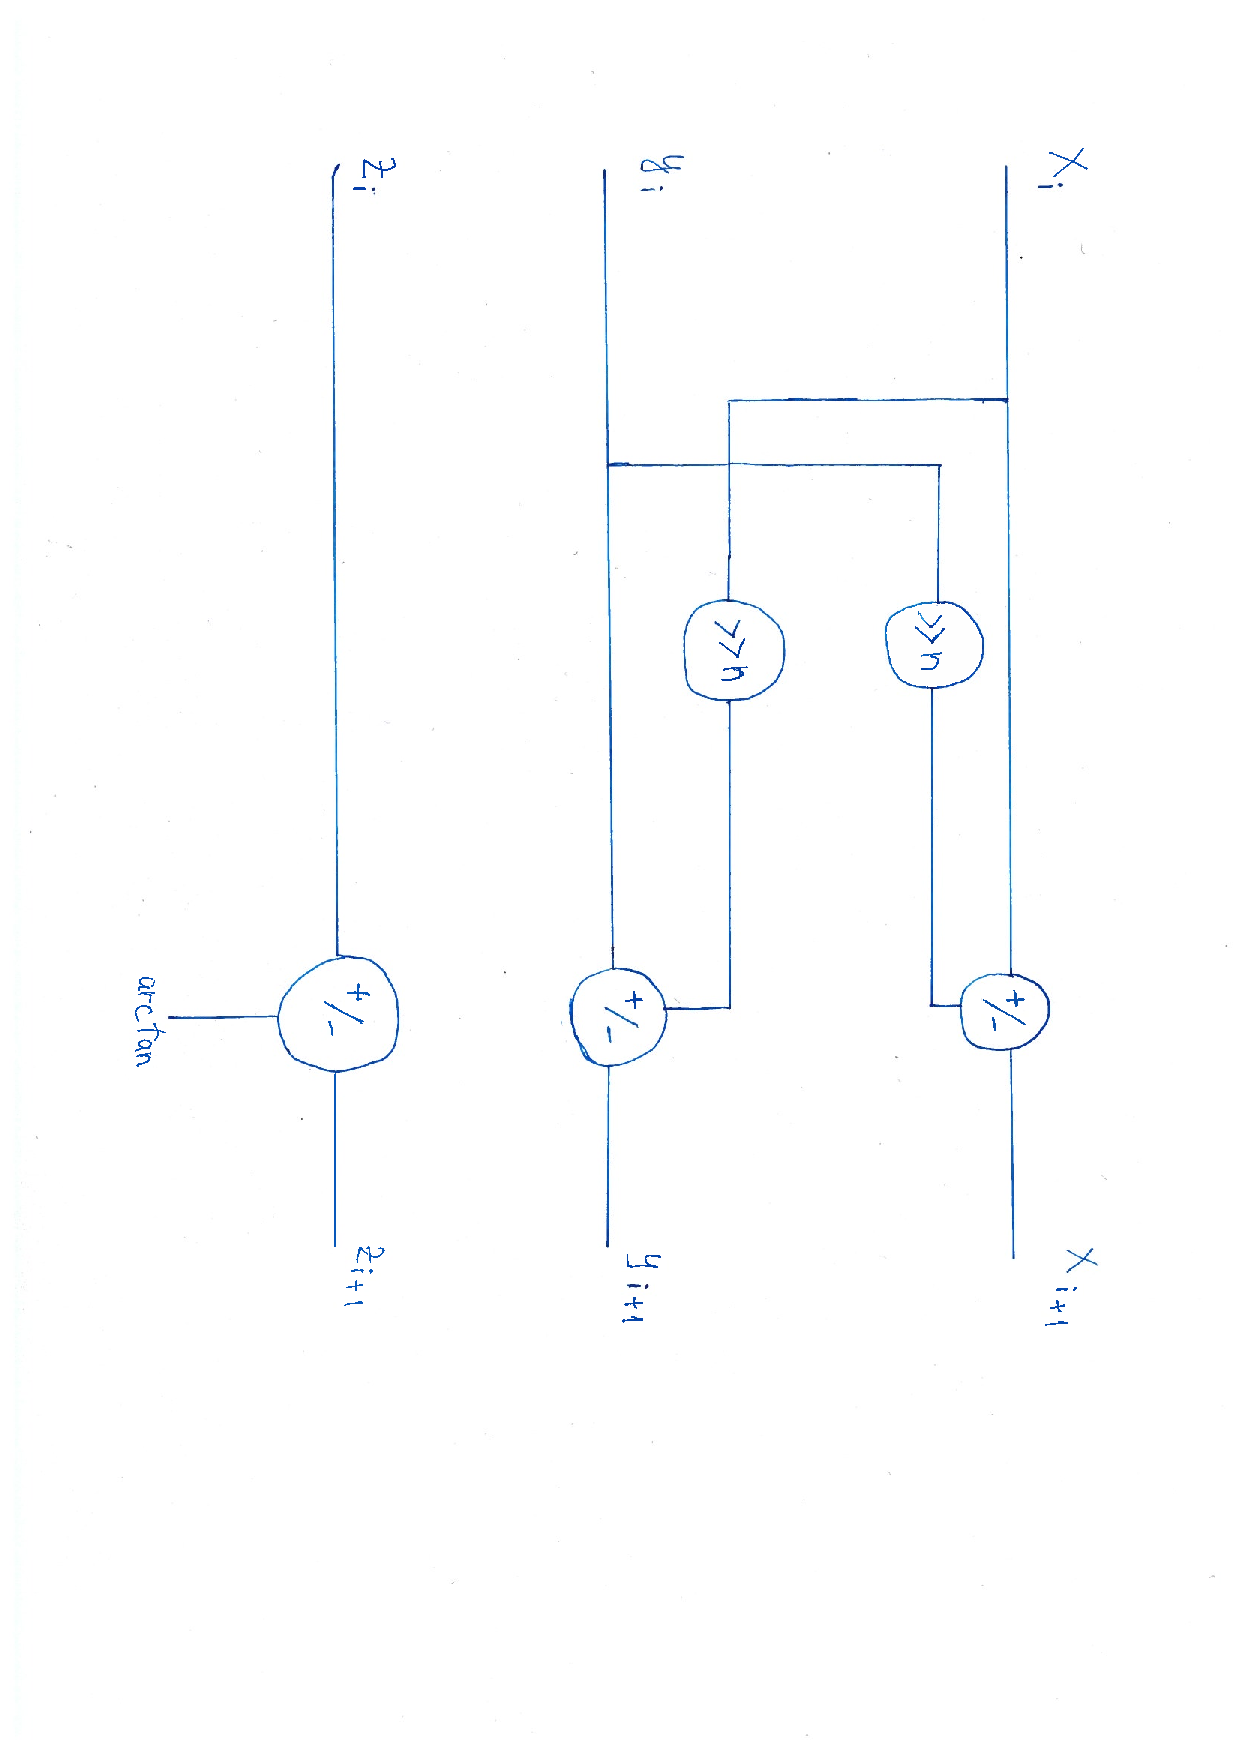
\includegraphics[clip, trim=2cm 7cm 2.2cm 2.5cm, width = 10cm,angle=90]{cordic_dfg.pdf}
	\caption{Data flow graph for CORDIC}
	\label{fig:cordic_dfg}
\end{figure}

The two shift operations ($>>n$) represent the $2^{-i}$ part of each transfer 
function. This has to be controlled by $i$. The same applies for the to 
additions, for computing $x_{i+1}$ and $y_{i+1}$, which will in fact 
either add or subtract the result of the shift, based on $z_i$. These aspects
will be analysed in \ref{ssec:fsdm}. $z_i$ relies on a table containing the 
values of precomputed values for $arctan$. This is stored in memory, and will
contain the as many values, as the number of iterations the CORDIC algorithm 
is designed to take.

\subsection{Precedence graph (PG)}
The precedence graph
\begin{figure}[H]
	\centering
	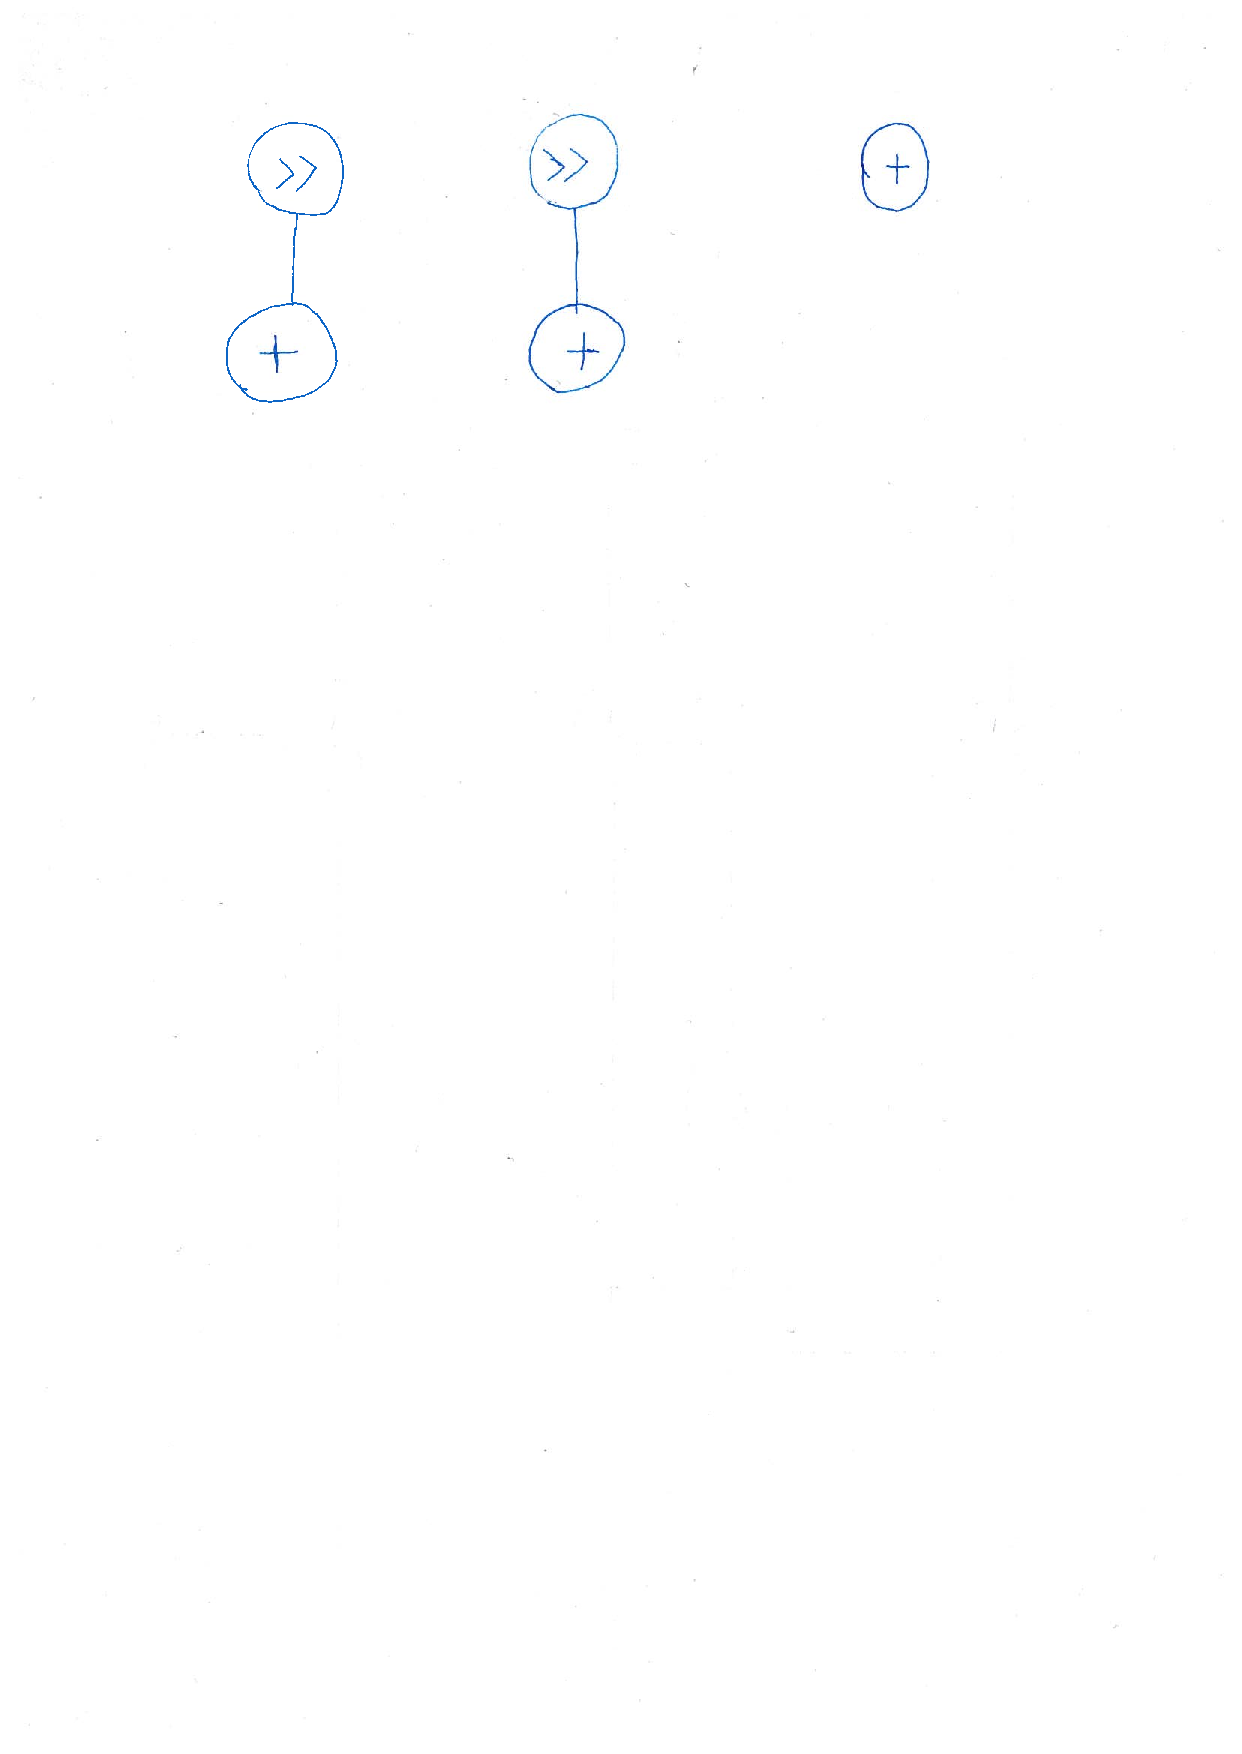
\includegraphics[width = \linewidth,trim=0 22.9cm 0 2cm, clip]{sequencediagram.pdf}
	\caption{Precedence graph for CORDIC}
	\label{fig:cordic_pg}
\end{figure}

\subsection{Hardware mapping}

\begin{figure}[H]
	\centering
	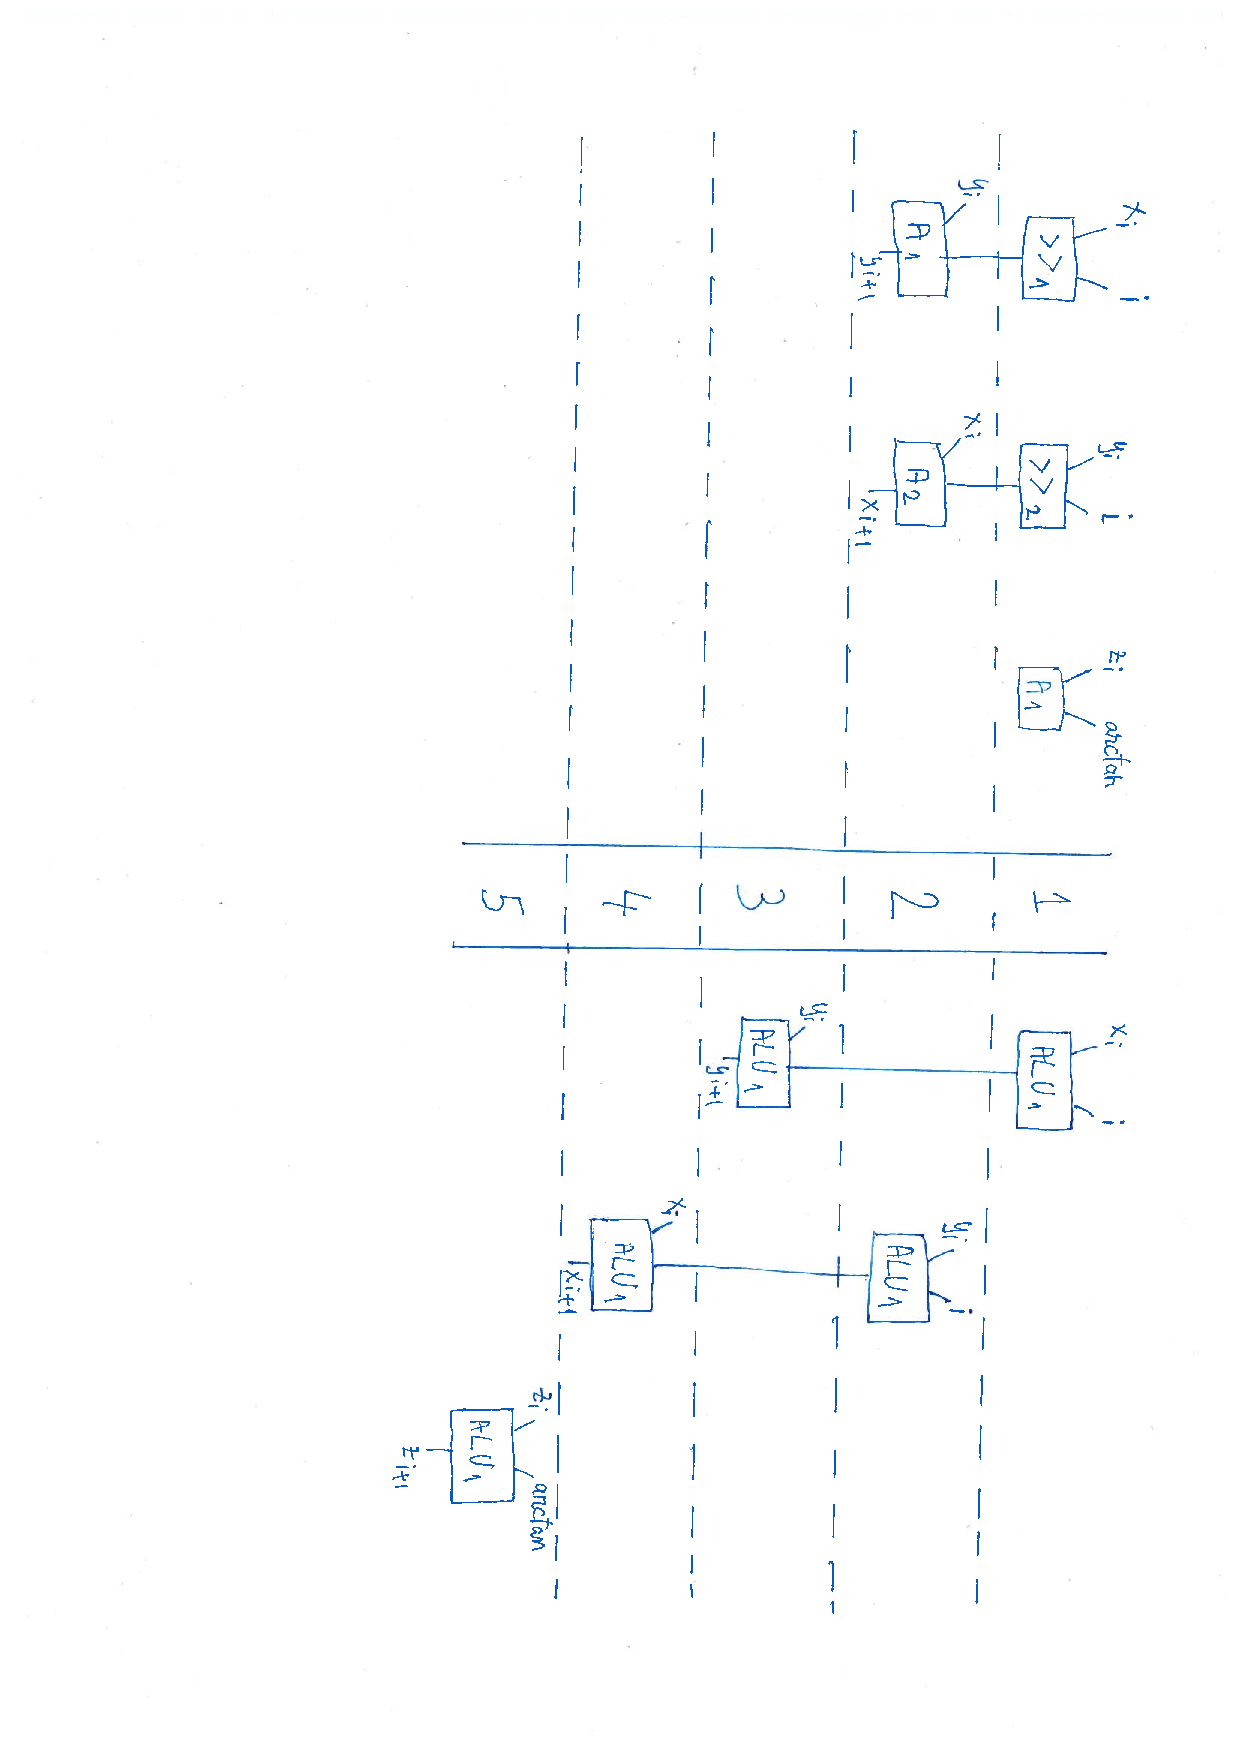
\includegraphics[height = \textwidth,angle=91, trim=6.5cm 3.5cm 1.5cm 3cm, clip]{schedules.pdf}
	\caption{1:1 hardware mapping, and fully shared ALU for CORDIC}
	\label{fig:schedules}
\end{figure}
	

\begin{figure}[H]
	\centering
	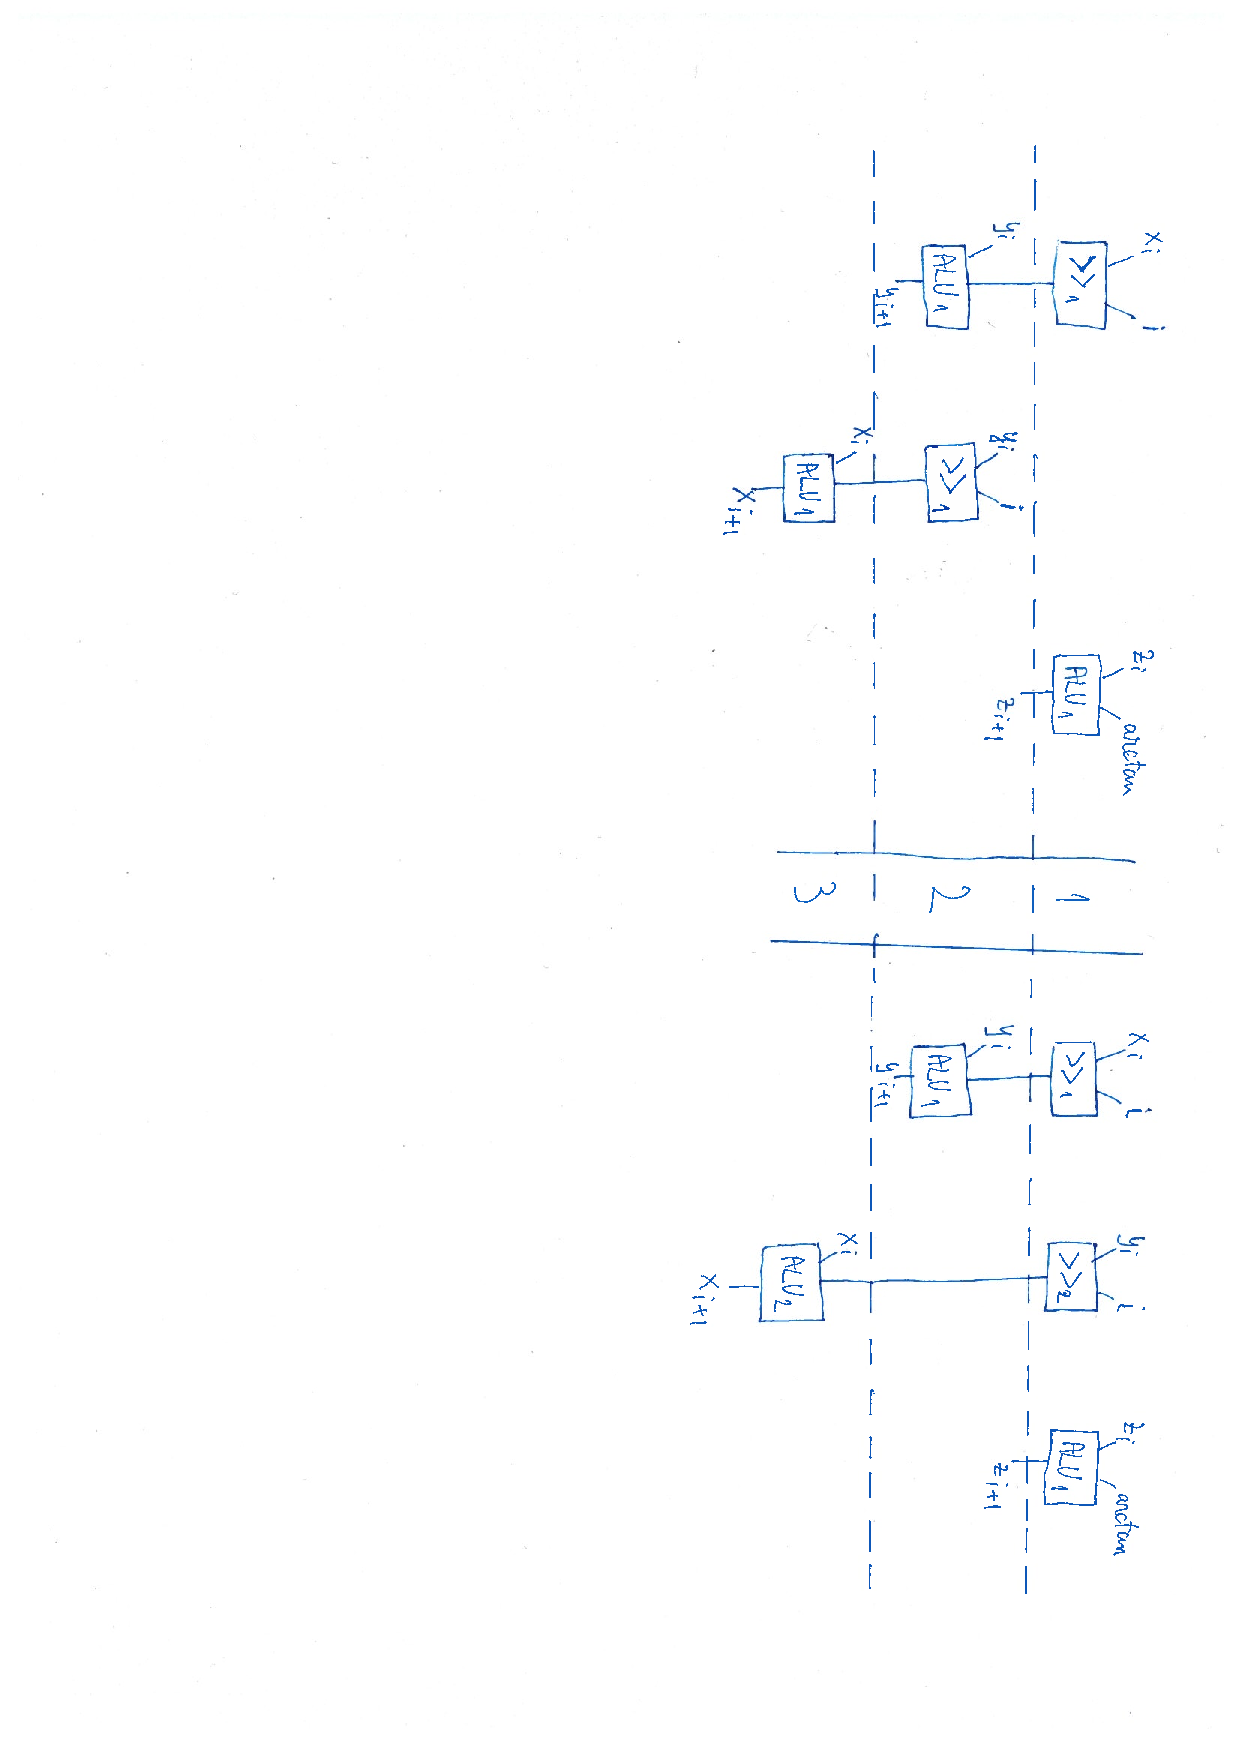
\includegraphics[height = \textwidth,angle=91, trim=7cm 5cm 1.5cm 5cm]{schedules_1.pdf}
	\caption{Middle ground for hardware mapping for CORDIC}
	\label{fig:schedules_1}
\end{figure}

\subsection{Finite state machine with data path (FSDM)}\label{ssec:fsdm}

\begin{figure}[H]
	\centering
	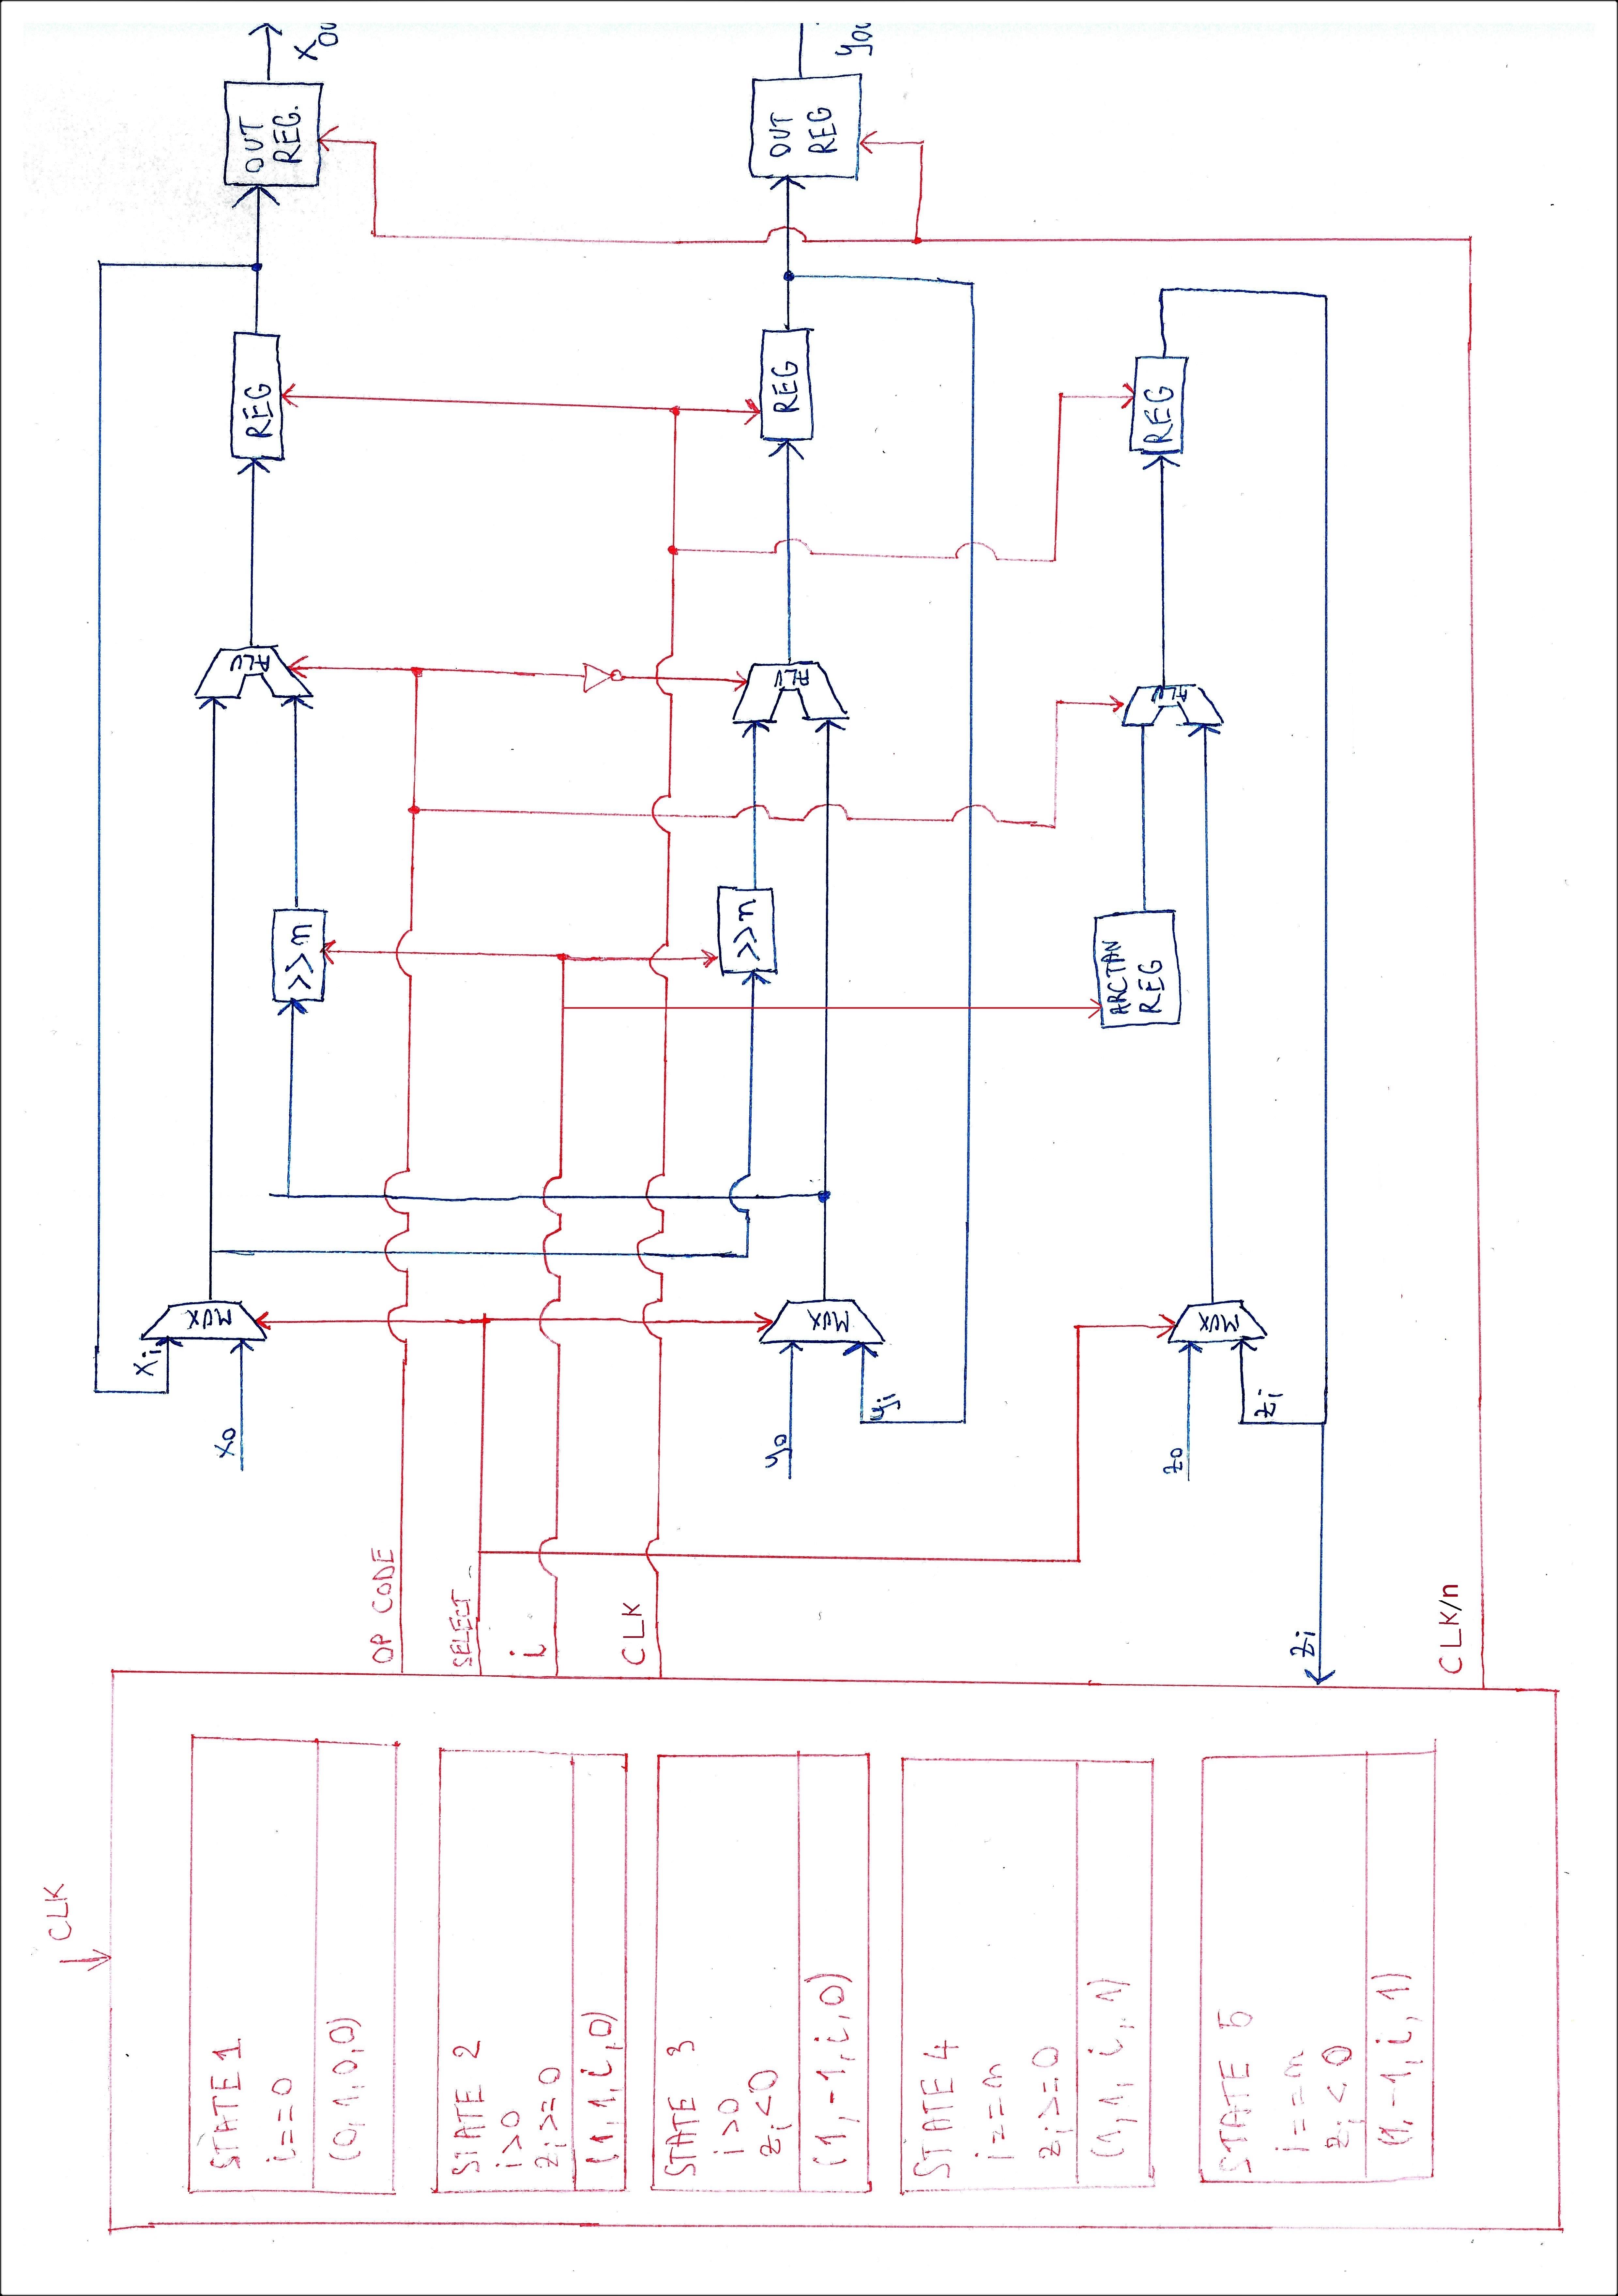
\includegraphics[width = \linewidth]{finite_state_machine_edit.jpg}
	\caption{Finite State Machine with Data Path}
	\label{fig:finite_state_machine}
\end{figure}

\printbibliography

\end{document}